\chapter{Experimenteller Aufbau}
Die mit der \gls{pxs} erzeugte Strahlung wird mit der \gls{rzp} in einer Entfernung von \SI{4}{\meter} fokussiert. Die \gls{pxs} wird mit einem Rohr, in dem der Strahl propagiert, zur Vakuumkammer verbunden. In dem gesamten System wird ein Druck von ca. \SI{2e6}{\meter\bar} aufrechterhalten. In der Vakuumkammer werden der vertikale Spalt mit verstellbarer Spalthöhe, der Probenhalter und der \gls{moench03} im Strahlengang installiert.

\noindent
Die Probe im Strahlengang wird \SI{160}{\milli\meter} hinter dem Fokuspunkt der \gls{rzp} positioniert. Der Detektor wird $l = \SI{607(7)}{\milli\meter}$ von der Probe entfernt befestigt. In Hinblick auf die Sensorgröße \qtyproduct{10 x 10}{\milli\meter} des \gls{moench03} können die Streuwinkel $2\theta$ bis \SI{0.47}{\degree} beobachtet werden, welche mit der $\lambda_\text{Gd ,M5} = \SI{1.045}{\nano\meter}$ die Streuvektoren bis \SI{49,5}{\per\micro\meter} vermessen lässt.
\begin{figure}[H]
    \centering
    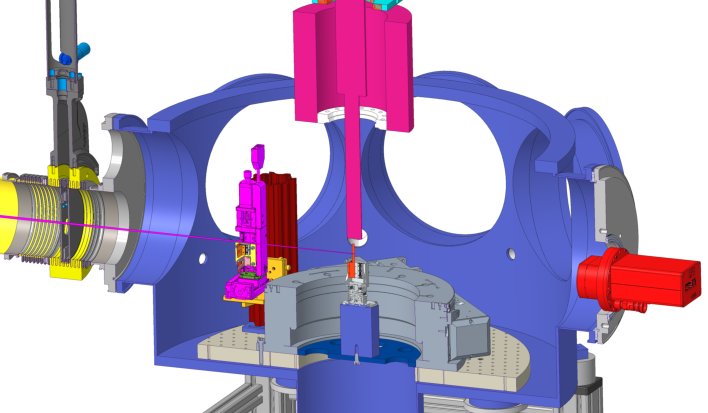
\includegraphics{images/aufbau/aufbau_empty.pdf}
    \caption{Die Skizze des Messaufbaus. Die Einzelbauteile sind farbig kodiert. Das Rohr (gelb) verbindet die Vakuumkammer (blau) mit der \gls{pxs}. Der horizontale Spalt (fuchsia) dient zum Abschneiden des gewünschten Bereichs der Strahlsanduhr. Der Probenhalter (pink) lässt sich seitlich bewegen, rotieren und vertikal hoch und herunterfahren. Die Spaltposition sowie die Spalthöhe lassen sich frei variieren. Der MÖNCH-Detektor (rot) ist an der zum Strahlgang (gelb) gegenüberliegenden Wand der Vakuumkammer befestigt.}
    \label{fig:anlage}
\end{figure}
\noindent
Mit Rücksicht auf die fast doppelt so hohe erwartete Streuungsintesität (s. Abb. \ref{fig:proben_vergleich_centered}) und höheres Ein-Photon-Signal im Gegensatz zur Photonenenergie $h\nu_\text{Fe, L3}$ werden die Messungen im Rahmen dieser Arbeit lediglich an der Photonenenergie $h\nu_\text{Gd, M5}$ durchgeführt.

% \noindent
% In der ersten Näherung kann die Domänenstruktur der Probe \textbf{DS220126} als ein Gitter betrachtet werden, wobei die Domänengröße dem Spaltabstand $d$ entspricht. Dieser kann mit den MFM-Aufnahmen (Abb. \ref{fig:mfm-amplitude-ft}c)) mit ca. \SI{300}{\nano\meter} abgeschätzt werden. In Hinblick darauf, dass die Streuung in der aktuellen Transmissionsgeometrie unter den kleinen Winkeln beobachtet wird, lässt sich der Abstand des $k$-ten Maximums zum $0$-ten Maximum wie folgt ermitteln
% \begin{equation}
%      r_{k} = \frac{kl\lambda}{d},
%  \end{equation}
%  wobei $l = \SI{607(6)}{\milli\meter}$ - Abstand vom Gitter bis zur Beobachtungsfläche und $\lambda$ - Photonenwellenlänge. Die Photonenenergie $h\nu_{\text{Gd, M5}} = \SI{1184,79}{\eV}$ entspricht der Wellenlänge $\lambda_{\text{Gd, M5}} = \SI{1,05}{\nano\meter}$. So ist der erwartete Abstand des 1. Streuringes bis zum $0$-ten Hauptmaxima 
%  \begin{equation}
%      r_{1, \text{ Gd, M5}} = \frac{1 \cdot l\lambda_{\text{Gd, M5}}}{d} = \SI{2.12(2)}{\milli\meter}.
%      \label{eq:theo_r1}
% \end{equation}
\noindent
Die Dunkelbilder, die später aus den Aufnahmen subtrahiert wurden (s. Abschnitt \ref{text:moench_theorie}), wurden alle 30 Minuten in Stückzahl \num{10000} aufgenommen, um die zeitliche Entwicklung des Hintergrundrauschens mitzunehmen. Ein kontinuierlicher Aufnahmevorgang der \gls{pxs} kann höchstens bis \SI{20}{\second} dauern. Die Pulsfrequenz $f_\text{\gls{pxs}}$ ist konstant und beträgt \SI{100}{\hertz}. So werden es \num{2000} Pulsen innerhalb eines \SI{20}{\second} Aufnahmevorgangs emittiert. Jedem Puls geht ein Triggersignal voraus, das \SI{1}{\milli\second} vor dem Puls generiert wird.

\noindent
Der \gls{moench03} hat eine einstellbare Verzögerung zwischen dem Aufnahmestart und dem Triggersignaleingang. Diese wird so konfiguriert, dass der \SI{10}{\pico\second} Puls der \gls{pxs} vollständig in das Belichtungszeitfenster $\tau$ hineinpasst. Gleichzeitig muss aber ein gewisser Jitter zwischen dem Triggergenerator und dem \gls{moench03} von einigen \SI{10}{\nano\second} beachtet werden. Aus diesem Grund konnte die Belichtungszeit $\tau$ unter der Bedingung, dass jeder Puls vollständig in jeder Aufnahme aufgenommen wird, höchstens bis auf \SI{1}{\micro\second} heruntergesetzt werden.

\noindent
Durch die Verkleinerung der Spalthöhe lässt sich ein kleinerer Energiebereich um die Resonanzenergie, der auf die Probe abgebildet wird, selektieren und die nichtresonanten Energien abschneiden, wodurch die Überlagerung des Direktstrahls mit dem Streuring vermieden werden soll und eine bessere Energieauflösung erreichbar ist. Die Beugung an den Spaltkanten kann sich jedoch mit der Beugung an der Probe überlagern und nicht davon trennbar sein. Aus diesem Grund wurden die Messungen sowohl mit dem schmal eingestellten Spalt als auch ohne den Spalt durchgeführt.

\noindent
Neben der Strahlung im Röntgenspektrum treten bei der \gls{pxs} auch Strahlung im sichtbaren Spektrum, Streuung des einfallenden Laserlichts und Elektronenemission auf. Obwohl der Sensor von \gls{moench03} eine \SI{500}{\nano\meter} Al-Beschichtung hat, scheint der Detektor vom Rand her ungeschützt zu sein. So wurden die Pixel am Rand des Detektors ständig belichtet. Es wurde daher zusätzlich im Strahlengang eine Mylar-Folie mit \SI{200}{\nano\meter} Al-Beschichtung installiert, die die Intensität des sichtbaren und infraroten Lichtes deutlich abschwächte. Obwohl die Elektronen mit einem starken Magneten vom Strahlengang großteils abgelenkt werden, konnten einige Elektronen auf dem \gls{moench03} detektiert werden. In den Experimenten hat sich gezeigt, dass der installierte Filter ihre Anzahl jedoch reduzierte.
%
% \noindent
% Könnte die Belichtungszeit $\tau$ auf \SI{100}{\nano\second} gesetzt werden, ließ sich die Standardabweichung $\sigma$ von ca. \SI{21}{\adu} bis \SI{19}{\adu} senken. So würde das ursprüngliche \gls{snr} immer noch im Bereich von 7-\SI{10}{\decibel} liegen.

\noindent
Die resonante magnetische Streuung tritt am stärksten nur im schmalen Bereich um die Resonanzenergien $h\nu_{\text{Fe, L3}}$ bzw. $h\nu_{\text{Gd, M5}}$ auf. Diese Energien sind aber nicht die Zielenergien der \gls{rzp} für Fe und Gd. Aus diesem Grund muss der Strahl mit dem Fokuspunkt vertikal verschoben werden, damit die Resonanzenergie mittig auf dem Detektor liegt. Die Effizienz und die Abbildungsschärfe der \gls{rzp}, also die Energieauflösung pro Längeneinheit entlang der Energieachse, sind jedoch maximal an der Zielenergie und nehmen mit dem Abstand zur Zielenergie ab.

\noindent
In Abschnitt \ref{text:quelle_roentgen} wurde der detektierte Photonenfluss ohne Probe der \gls{pxs} abgeschätzt. In Hinblick auf die niedrige erwartete Transmissionsrate der Probe \textbf{DS220126} (Abb. \ref{fig:proben_vergleich_centered}) wurde der Photonenfluss, der schließlich nach der Streuung an der Probe detektiert wird, erneut experimentell bestimmt. Dieses Verfahren ist in Abschnitt \ref{text:streuung_counting} detailliert präsentiert.

\noindent
Der detektierte Photonenfluss an der Probe konnte mit \SI{60(5)}{\photons} pro Puls abgeschätzt werden, wobei ca. \SI{45(5)}{\photons} im Direktstrahl liegen. Es werden insgesamt von \num{40000} bis \SI{50000}{\captures} Pulse aufgenommen, um ausreichend Streusignal in der 1. Ordnung des Streumusters zu detektieren.


% 2 "PXS wird mit der Vakuumkammer verbunden" stellt es so dar, als sei die PXS selbst nicht im Vakuum. Gleiches Zeile 9
% 2 vertikaler Spalt ist eigentlich horizontal, oder?
% 9 "Der Probenhalter (pink) lässt sich seitlich bewegen, rotieren und vertikal hoch und herunterfahren. Die Spaltposition sowie die Spalthöhe lassen sich frei variieren." Was mich daran stört: Probenhalter erst linear quer zum Strahl, dann rotierbar, dann auch in der Höhe linear fahrbar (Reihenfolge der Achsen). Und der Spalt lässt sich "frei variieren", naja im Rahmen gewisser Grenzen. ->Gegenvorschlag: Der Probenhalter (pink) ist in zwei Richtungen senkrecht zum Strahl motorisiert linear positionierbar sowie um die vertikale Achse rotierbar. Öffnungsweite und Position des Spaltes sind ebenfalls motorisiert einstellbar.


% 44 letztes Wort "präsentiert" gefällt mir da nicht wirklich. Vorgestellt, dargelegt, dargestellt, ... also schon vom englischen "to present", aber nicht so tadaaa-mäßig ;)
